% ============================================================
% Reporte: Producto Punto de Vectores en Ensamblador x86 con FPU
% Autor: Edson Joel Carrera Avila
% ============================================================

\documentclass[12pt, letterpaper]{article}

\usepackage[utf8]{inputenc}
\usepackage[T1]{fontenc}
\usepackage[english]{babel}
\usepackage{geometry}
\usepackage{graphicx}
\usepackage{listings}
\usepackage{xcolor}
\usepackage{booktabs}
\usepackage{amsmath}
\usepackage{hyperref}
\usepackage{fancyhdr}
\usepackage{float}
\usepackage{caption}
\usepackage{tikz}
\usetikzlibrary{shapes.geometric, arrows.meta, positioning}

\geometry{top=2.5cm, bottom=2.5cm, left=3cm, right=2.5cm}

% --- Colores y estilo de código ---
\definecolor{codegray}{rgb}{0.95,0.95,0.95}
\definecolor{codegreen}{rgb}{0.0,0.5,0.0}
\definecolor{codeblue}{rgb}{0.0,0.0,0.65}
\definecolor{codepurple}{rgb}{0.45,0.0,0.55}

\lstdefinelanguage{MASM}{
    morekeywords={PROC,ENDP,END,PUSH,POP,MOV,ADD,SUB,CALL,RET,JMP,
                  JE,JB,JA,JLE,JNZ,DEC,INC,CMP,TEST,EXTERN,
                  BYTE,DWORD,QWORD,PTR,
                  EBP,ESP,ESI,EDI,ECX,EAX,AL,ST,
                  FLD,FLDZ,FSTP,FXCH,FMUL,FADDP,
                  .586,.model,.data,.code,flat,c},
    sensitive=false,
    morecomment=[l]{;}
}

\lstdefinelanguage{CPP}{
    morekeywords={int,double,cout,cin,endl,using,namespace,std,extern,
                  include,return,for,vector,data},
    sensitive=true,
    morecomment=[l]{//},
    morestring=[b]"
}

\lstset{
    backgroundcolor=\color{codegray},
    basicstyle=\ttfamily\footnotesize,
    keywordstyle=\color{codeblue}\bfseries,
    commentstyle=\color{codegreen}\itshape,
    numbers=left, numberstyle=\tiny\color{gray}, numbersep=8pt,
    frame=single, rulecolor=\color{gray!50},
    breaklines=true, captionpos=b, tabsize=4,
    showstringspaces=false,
    literate=
        {á}{{\'a}}1 {é}{{\'e}}1 {í}{{\'i}}1 {ó}{{\'o}}1 {ú}{{\'u}}1
        {Á}{{\'A}}1 {É}{{\'E}}1 {Í}{{\'I}}1 {Ó}{{\'O}}1 {Ú}{{\'U}}1
        {ñ}{{\~n}}1 {Ñ}{{\~N}}1
}

% --- Encabezado ---
\pagestyle{fancy}
\fancyhf{}
\rhead{Práctica 05}
\lhead{\textit{Edson Joel Carrera Avila}}
\cfoot{\thepage}
\renewcommand{\headrulewidth}{0.5pt}

% ============================================================
\begin{document}

% --- Portada ---
\begin{titlepage}
    \centering
    \vspace*{1.5cm}

    {\Large \textbf{Universidad Autónoma de la Ciudad de México}}\\[0.3cm]
    {\large Licenciatura en Ingeniería de Software}\\[0.2cm]
    {\large Arquitectura de Computadoras}\\[2.5cm]

    \rule{\linewidth}{0.5pt}\\[0.4cm]
    {\LARGE \bfseries Práctica 05}\\[0.3cm]
    {\Large Producto Punto de Vectores en Ensamblador x86}\\[0.3cm]
    \rule{\linewidth}{0.5pt}\\[2cm]

    \begin{flushleft}
        \textbf{Alumno:} Edson Joel Carrera Avila \\[0.3cm]
        \textbf{Grupo:} 302 \\[0.3cm]
        \textbf{Profesor:} Prof. Mtro. Omar Nieto Crisóstomo \\[0.3cm]
        \textbf{Fecha:} \today
    \end{flushleft}
    \vfill
\end{titlepage}

\tableofcontents
\newpage

% ============================================================
\section{Introducción}

Esta práctica consiste en implementar la operación de \textbf{producto punto} (también llamado producto escalar o \textit{dot product}) entre dos vectores de números reales, utilizando \textbf{lenguaje ensamblador x86} con la \textbf{Unidad de Punto Flotante (FPU)}. La función ensamblador es invocada desde un programa principal escrito en \textbf{C++}, que se encarga de solicitar los datos al usuario y mostrar el resultado.

El objetivo no es únicamente reproducir la operación matemática, sino entender cómo el procesador accede a arreglos en memoria mediante punteros, cómo recorre estructuras de datos con registros de índice, y cómo acumula resultados de punto flotante usando la pila interna de la FPU.

\subsection*{¿Qué es el producto punto?}

Dados dos vectores $\vec{u} = (u_1, u_2, \ldots, u_N)$ y $\vec{v} = (v_1, v_2, \ldots, v_N)$ de la misma dimensión $N$, el producto punto se define como la suma de los productos elemento a elemento:

\begin{equation}
    \vec{u} \cdot \vec{v} = \sum_{i=1}^{N} u_i \cdot v_i = u_1 v_1 + u_2 v_2 + \cdots + u_N v_N
\end{equation}

El resultado es un \textbf{escalar} (un único número), razón por la cual también se llama producto escalar. Por ejemplo, para vectores de dimensión 3:

\begin{equation}
    (2,\; 3,\; 4) \cdot (1,\; 5,\; 2) = (2 \times 1) + (3 \times 5) + (4 \times 2) = 2 + 15 + 8 = 25
\end{equation}

\subsection*{¿Cómo se representan los vectores en memoria?}

En C++, un \texttt{vector<double>} almacena sus elementos de forma \textbf{contigua} en memoria. Cada elemento de tipo \texttt{double} ocupa \textbf{8 bytes} (64 bits). Si el primer elemento está en la dirección $D$, los elementos están en:

\begin{table}[H]
    \centering
    \begin{tabular}{@{}ccc@{}}
        \toprule
        \textbf{Elemento} & \textbf{Dirección} & \textbf{Desplazamiento} \\
        \midrule
        \texttt{vec[0]} & $D$       & $+0$ bytes \\
        \texttt{vec[1]} & $D + 8$   & $+8$ bytes \\
        \texttt{vec[2]} & $D + 16$  & $+16$ bytes \\
        \texttt{vec[i]} & $D + 8i$  & $+8i$ bytes \\
        \bottomrule
    \end{tabular}
    \caption{Distribución en memoria de un arreglo de \texttt{double}}
\end{table}

El ensamblador recorre estos elementos avanzando el puntero en 8 bytes por iteración con la instrucción \texttt{ADD ESI, 8}.

% ============================================================
\section{Organización del proyecto}

El proyecto consta de dos archivos que trabajan en conjunto:

\begin{table}[H]
    \centering
    \begin{tabular}{@{}lp{9cm}@{}}
        \toprule
        \textbf{Archivo} & \textbf{Función} \\
        \midrule
        \texttt{productoPunto.asm} & Implementa en ensamblador x86 la función \texttt{productoPunto}, que recibe punteros a los dos vectores y su dimensión, y devuelve el escalar resultante. \\
        \texttt{main.cpp}          & Programa principal en C++ que solicita los datos al usuario, llena los vectores y llama a la función ensamblador. \\
        \bottomrule
    \end{tabular}
    \caption{Archivos del proyecto}
\end{table}

La directiva \texttt{.model flat, c} y la declaración \texttt{extern "C"} en C++ garantizan la compatibilidad de nombres entre ambos módulos. El resultado de tipo \texttt{double} se retorna en \texttt{ST(0)} de la FPU, conforme a la convención \textit{cdecl} de x86.\\

El núcleo del algoritmo es un bucle de cuatro fases que se repite $N$ veces:

\begin{figure}[H]
    \centering
    \resizebox{0.75\textwidth}{!}{%
        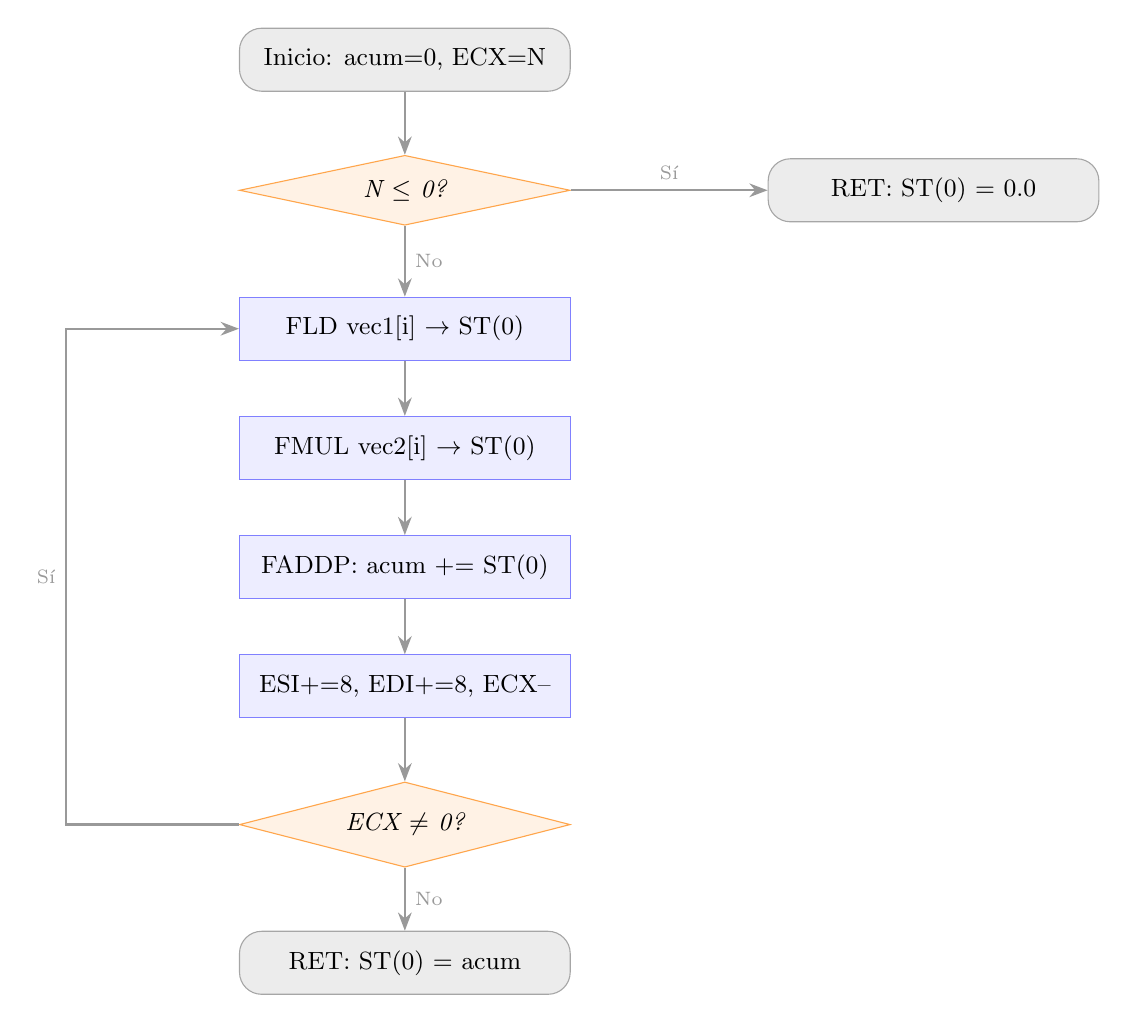
\begin{tikzpicture}[
            startstop/.style={rectangle, rounded corners=8pt, draw=gray!70, fill=gray!15,
                              minimum width=4.2cm, minimum height=0.8cm, font=\small},
            process/.style  ={rectangle, draw=blue!50, fill=blue!7,
                              minimum width=4.2cm, minimum height=0.8cm, font=\small},
            decision/.style ={diamond, aspect=2.5, draw=orange!70, fill=orange!10,
                              minimum width=4.2cm, font=\small\itshape, inner sep=2pt},
            arr/.style      ={-Stealth, thick, gray!80}
        ]
            \node[startstop] (ini)   {Inicio: acum=0, ECX=N};
            \node[decision,  below=0.8cm of ini]   (test)  {N $\leq$ 0?};
            \node[process,   below=0.9cm of test]  (fld)   {FLD vec1[i] $\to$ ST(0)};
            \node[process,   below=0.7cm of fld]   (fmul)  {FMUL vec2[i] $\to$ ST(0)};
            \node[process,   below=0.7cm of fmul]  (fadd)  {FADDP: acum += ST(0)};
            \node[process,   below=0.7cm of fadd]  (adv)   {ESI+=8, EDI+=8, ECX--};
            \node[decision,  below=0.8cm of adv]   (jnz)   {ECX $\neq$ 0?};
            \node[startstop, below=0.8cm of jnz]   (fin)   {RET: ST(0) = acum};
            \node[startstop, right=2.5cm of test]  (ret0)  {RET: ST(0) = 0.0};

            \draw[arr] (ini)  -- (test);
            \draw[arr] (test) -- node[right, font=\scriptsize]{No} (fld);
            \draw[arr] (test) -- node[above, font=\scriptsize]{Sí} (ret0);
            \draw[arr] (fld)  -- (fmul);
            \draw[arr] (fmul) -- (fadd);
            \draw[arr] (fadd) -- (adv);
            \draw[arr] (adv)  -- (jnz);
            \draw[arr] (jnz)  -- node[right, font=\scriptsize]{No} (fin);
            \draw[arr] (jnz.west) -- ++(-2.2,0) |- node[near start, left, font=\scriptsize]{Sí} (fld.west);
        \end{tikzpicture}%
    }
    \caption{Diagrama de flujo del algoritmo de producto punto}
\end{figure}

Paso a paso por iteración:

\begin{enumerate}
    \item \textbf{\texttt{FLD QWORD PTR [ESI]}}: carga el elemento \texttt{vec1[i]} al tope de la FPU (\texttt{ST(0)}), empujando el acumulador a \texttt{ST(1)}.
    \item \textbf{\texttt{FMUL QWORD PTR [EDI]}}: multiplica \texttt{ST(0)} por \texttt{vec2[i]} sin hacer \textit{pop}; el resultado ($\texttt{vec1[i]} \times \texttt{vec2[i]}$) queda en \texttt{ST(0)}.
    \item \textbf{\texttt{FADDP ST(1), ST(0)}}: suma \texttt{ST(0)} al acumulador en \texttt{ST(1)}, hace \textit{pop} de \texttt{ST(0)}, y el acumulador actualizado queda en \texttt{ST(0)}.
    \item \textbf{\texttt{ADD ESI, 8 / ADD EDI, 8}}: avanza ambos punteros al siguiente elemento del arreglo.
    \item \textbf{\texttt{DEC ECX / JNZ bucle}}: decrementa el contador; si no llegó a cero, repite.
\end{enumerate}

% ============================================================
\section{Código fuente}

\subsection{Código C++ (main.cpp)}

\begin{lstlisting}[language=CPP, caption={\texttt{main.cpp} --- Programa en C++ que invoca la función ensamblador}]
#include <iostream>
#include <vector>
using namespace std;

extern "C" double productoPunto(double* vec1, double* vec2, int N);

int main() {
    int n;
    cout << "Ingresa la dimension de los vectores (N): ";
    cin >> n;

    vector<double> vec1(n);
    vector<double> vec2(n);

    cout << "\n--- DATOS DEL VECTOR 1 ---" << endl;
    for (int i = 0; i < n; i++) {
        cout << "Ingresa el valor para vec1[" << i << "]: ";
        cin >> vec1[i];
    }

    cout << "\n--- DATOS DEL VECTOR 2 ---" << endl;
    for (int i = 0; i < n; i++) {
        cout << "Ingresa el valor para vec2[" << i << "]: ";
        cin >> vec2[i];
    }

    double resultado = productoPunto(vec1.data(), vec2.data(), n);

    cout << "\n----------------------------------------\n";
    cout << "Resultado del Producto Punto: " << resultado << endl;

    return 0;
}
\end{lstlisting}

\subsection{Código ensamblador (productoPunto.asm)}

\begin{lstlisting}[language=MASM, caption={\texttt{productoPunto.asm} --- Cálculo del producto punto con la FPU}]
; ============================================================
; Autor: Edson Joel Carrera Avila
; productoPunto.asm
; ============================================================

.586
.model flat, c

.code

; Parametros: [EBP+8]  = puntero a vec1 (double*)
;             [EBP+12] = puntero a vec2 (double*)
;             [EBP+16] = N (int)
productoPunto PROC
    PUSH    EBP                  ; Guardar marco de pila anterior
    MOV     EBP, ESP             ; Establecer nuevo marco de pila
    PUSH    ESI                  ; Preservar ESI (convencion cdecl)
    PUSH    EDI                  ; Preservar EDI (convencion cdecl)
    MOV     ESI, [EBP+8]         ; ESI = puntero al inicio de vec1
    MOV     EDI, [EBP+12]        ; EDI = puntero al inicio de vec2
    MOV     ECX, [EBP+16]        ; ECX = N (contador del ciclo)
    FLDZ                         ; ST(0) = 0.0  (acumulador)
    TEST    ECX, ECX             ; Comparar N con 0
    JLE     fin                  ; Si N <= 0, retornar 0.0

bucle:
    FLD     QWORD PTR [ESI]      ; ST(0) = vec1[i], acum sube a ST(1)
    FMUL    QWORD PTR [EDI]      ; ST(0) = vec1[i] * vec2[i]
    FADDP   ST(1), ST(0)         ; ST(1) = acum + producto; pop
    ADD     ESI, 8               ; Avanzar al siguiente double de vec1
    ADD     EDI, 8               ; Avanzar al siguiente double de vec2
    DEC     ECX                  ; Decrementar contador
    JNZ     bucle                ; Si ECX != 0, repetir

fin:
    POP     EDI
    POP     ESI
    MOV     ESP, EBP
    POP     EBP
    RET
productoPunto ENDP

END
\end{lstlisting}

% ============================================================
\section{Instrucciones x86 utilizadas}

\begin{table}[H]
    \centering
    \begin{tabular}{@{}lp{9.5cm}@{}}
        \toprule
        \textbf{Instrucción} & \textbf{Qué hace} \\
        \midrule
        \texttt{PUSH / POP} & Coloca o retira un valor de 32 bits de la pila del sistema; se usan para el prólogo/epílogo y para preservar registros. \\
        \texttt{MOV}   & Copia un valor entre registros o entre registro y memoria. \\
        \texttt{ADD}   & Suma un valor inmediato a un registro; aquí avanza los punteros 8 bytes por iteración. \\
        \texttt{DEC}   & Decrementa el operando en 1; actualiza las banderas (\textit{flags}) del procesador, permitiendo que \texttt{JNZ} las consulte. \\
        \texttt{TEST}  & Realiza una AND lógica entre dos operandos sin guardar el resultado; solo actualiza las banderas para verificar si \texttt{ECX} es cero. \\
        \texttt{JLE}   & Salta si el resultado de la comparación indica ``menor o igual'' (\textit{jump if less or equal}); protege el bucle cuando $N \leq 0$. \\
        \texttt{JNZ}   & Salta si el resultado no es cero (\textit{jump if not zero}); mantiene el bucle mientras \texttt{ECX} $\neq 0$. \\
        \texttt{RET}   & Retorna al llamador (C++); el resultado \texttt{double} queda en \texttt{ST(0)} de la FPU. \\
        \texttt{FLDZ}  & Carga la constante 0.0 al tope de la pila FPU (\texttt{ST(0)}); sirve para inicializar el acumulador. \\
        \texttt{FLD}   & Carga (\textit{push}) un valor \texttt{QWORD} (8 bytes / \texttt{double}) desde memoria al tope de la pila FPU. \\
        \texttt{FMUL}  & Multiplica \texttt{ST(0)} por el operando de memoria indicado; guarda el resultado en \texttt{ST(0)} sin \textit{pop}. \\
        \texttt{FADDP} & Suma \texttt{ST(0)} a \texttt{ST(i)} y hace \textit{pop} de \texttt{ST(0)}; el resultado queda en lo que era \texttt{ST(1)}. \\
        \bottomrule
    \end{tabular}
    \caption{Instrucciones de propósito general utilizadas}
\end{table}

% ============================================================
\section{El rol de los registros}

\subsection{Marco de pila y parámetros}

Al momento en que C++ invoca \texttt{productoPunto}, coloca los tres argumentos en la pila del sistema en orden inverso (de derecha a izquierda, convención \textit{cdecl}). Después del prólogo \texttt{PUSH EBP / MOV EBP, ESP}, el mapa de la pila queda:

\begin{table}[H]
    \centering
    \begin{tabular}{@{}ccc@{}}
        \toprule
        \textbf{Dirección} & \textbf{Contenido} & \textbf{Tipo} \\
        \midrule
        \texttt{[EBP+16]} & \texttt{N}     & \texttt{int} (4 bytes) \\
        \texttt{[EBP+12]} & \texttt{vec2}  & \texttt{double*} (4 bytes en x86) \\
        \texttt{[EBP+8]}  & \texttt{vec1}  & \texttt{double*} (4 bytes en x86) \\
        \texttt{[EBP+4]}  & dirección de retorno & — \\
        \texttt{[EBP+0]}  & EBP anterior   & — \\
        \bottomrule
    \end{tabular}
    \caption{Mapa del marco de pila al inicio de \texttt{productoPunto}}
\end{table}

Los registros \texttt{ESI} y \texttt{EDI} son \textbf{preservados} (\texttt{PUSH}/\texttt{POP}) porque la convención \textit{cdecl} exige que el llamado los restaure.

\subsection{Registros utilizados}

\begin{table}[H]
    \centering
    \begin{tabular}{@{}llp{7.5cm}@{}}
        \toprule
        \textbf{Registro} & \textbf{Rol} & \textbf{Descripción} \\
        \midrule
        \texttt{ESI} & Puntero índice fuente & Apunta al elemento actual de \texttt{vec1}; avanza 8 bytes por iteración. \\
        \texttt{EDI} & Puntero índice destino & Apunta al elemento actual de \texttt{vec2}; avanza 8 bytes por iteración. \\
        \texttt{ECX} & Contador & Almacena \texttt{N} y cuenta regresiva hasta 0; controla el bucle. \\
        \texttt{ST(0)} & Tope de la pila FPU & Valor temporal: producto \texttt{vec1[i] * vec2[i]} en cada iteración. \\
        \texttt{ST(1)} & Segundo registro FPU & Acumulador: suma parcial del producto punto. \\
        \bottomrule
    \end{tabular}
    \caption{Registros del procesador utilizados en \texttt{productoPunto}}
\end{table}

% ============================================================
\section{Ejemplo de ejecución}

Para los vectores $\vec{u} = (2,\; 3,\; 4)$ y $\vec{v} = (1,\; 5,\; 2)$, el cálculo esperado es:

\begin{equation}
    \vec{u} \cdot \vec{v} = (2 \times 1) + (3 \times 5) + (4 \times 2) = 2 + 15 + 8 = 25
\end{equation}

La tabla siguiente muestra cómo evoluciona el acumulador iteración a iteración:

\begin{table}[H]
    \centering
    \begin{tabular}{@{}ccccc@{}}
        \toprule
        \textbf{Iteración} & \textbf{vec1[i]} & \textbf{vec2[i]} & \textbf{Producto} & \textbf{Acumulador} \\
        \midrule
        0 (inicial) & —    & —    & —              & 0 \\
        1           & 2.0  & 1.0  & $2 \times 1=2$   & 2 \\
        2           & 3.0  & 5.0  & $3 \times 5=15$  & 17 \\
        3           & 4.0  & 2.0  & $4 \times 2=8$   & \textbf{25} \\
        \bottomrule
    \end{tabular}
    \caption{Evolución del acumulador para $\vec{u}=(2,3,4)$ y $\vec{v}=(1,5,2)$}
\end{table}

\begin{figure}[hbtp]
    \centering
    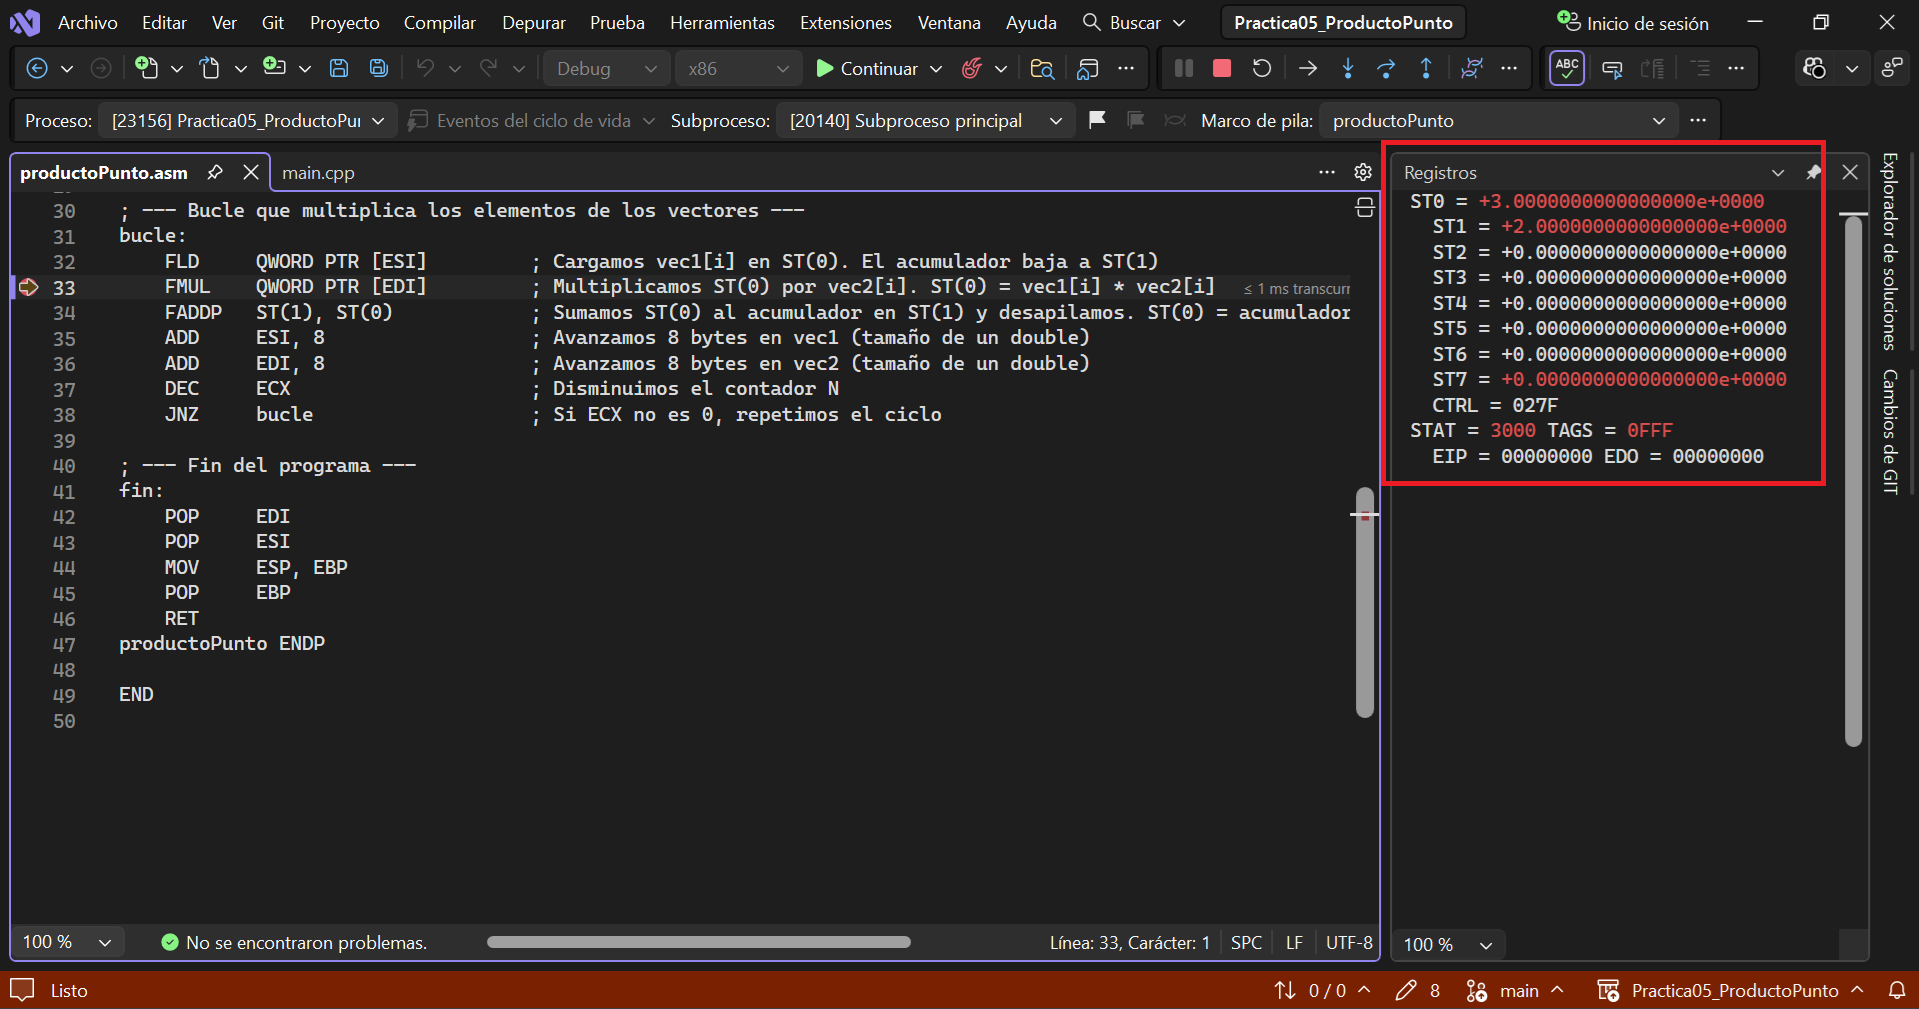
\includegraphics[width=0.7\textwidth]{fpu_registers_bucle.png}
    \caption{Registros moviendose en tiempo real}
    \label{fig:consola}
\end{figure}

La salida esperada en consola es:

\begin{figure}[hbtp]
    \centering
    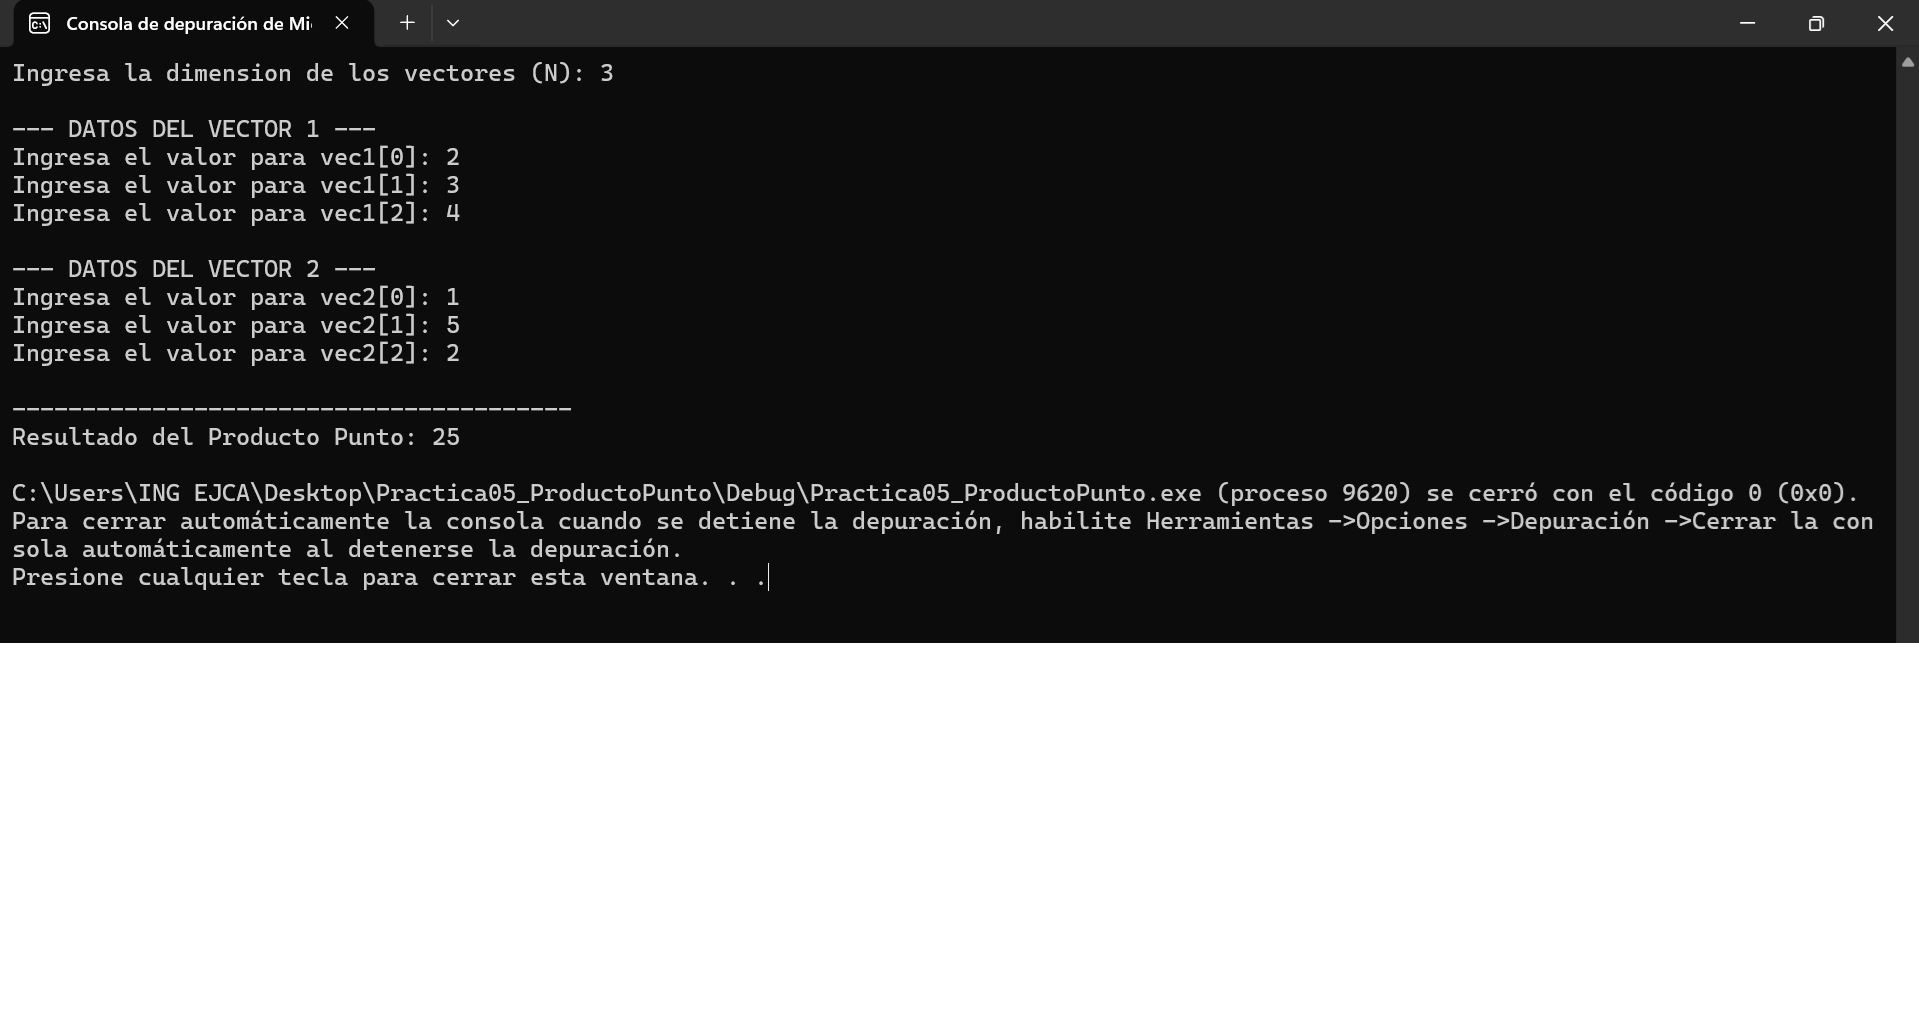
\includegraphics[width=0.7\textwidth]{consola_ejecucion.png}
    \vspace{-60pt}
    \caption{Salida del programa para $\vec{u}=(2,3,4)$ y $\vec{v}=(1,5,2)$}
    \label{fig:consola}
\end{figure}

% ============================================================
\section{Repositorio GitHub}

https://github.com/7mo-ArquitecturaComputadoras/Practica05\_ProductoPunto

% ============================================================
\section{Conclusiones}

\begin{itemize}
    \item El producto punto evidencia cómo el procesador \textbf{recorre arreglos en memoria mediante punteros}: avanzar \texttt{ESI} y \texttt{EDI} en 8 bytes por iteración es el equivalente ensamblador de incrementar un índice de arreglo en C++.
    \item El uso de \textbf{\texttt{FLDZ} como acumulador inicial} en la pila FPU es un patrón fundamental: cargar 0.0 antes del bucle garantiza que la primera suma sea correcta sin necesidad de un caso especial para $i = 0$.
    \item La instrucción \textbf{\texttt{FADDP}} combina suma y \textit{pop} en un solo ciclo de reloj, manteniendo la pila FPU con profundidad constante (un elemento, el acumulador) durante todo el bucle, lo cual es una práctica eficiente de gestión de la pila de punto flotante.
    \item La \textbf{verificación de $N \leq 0$} con \texttt{TEST} y \texttt{JLE} antes de entrar al bucle es una práctica de programación defensiva: sin ella, un contador negativo haría que \texttt{DEC} / \texttt{JNZ} ejecutaran el bucle $2^{32} - |N|$ veces, corrompiendo la memoria.
    \item Preservar \textbf{\texttt{ESI} y \texttt{EDI}} con \texttt{PUSH}/\texttt{POP} muestra el contrato de la convención \textit{cdecl}: el llamado es responsable de restaurar estos registros, garantizando que el código C++ no vea sus variables de iteración alteradas tras el retorno de la función ensamblador.
\end{itemize}

\end{document}
